\chapter{Model, cost, parameter learning, Gradient Descent }
Let us come back to the first example of \textit{price prediction} and formalize some aspects we have only mentioned. The objective here is to exploit this example to introduce and better clarify several concepts.\\
\section{Model representation}
At first, the training set we are using is something similar to the following:

\begin{table}[h]
    \centering
    \begin{tabular}{c c}
        \textbf{Size in feet$^2$($x$)}&\textbf{\color{red}Price(\$) in 1000's($y$)}\\
        \hline
        2104&460\\
        1416&232\\
        1534&315\\
        852&178\\
        ...&...
    \end{tabular}
\end{table}
\noindent
We will indicate with $m$ the number of samples of the training set (number of rows), $x$ is the input (possibly multivariate) variable, $y$ is the output variable, $(x,y)$ indicates generically a sample from the training set, while $(x^{(i)}, y^{(i)})$ indicates the $i$-th sample of the training set.

\begin{figure}[h]
    \centering
    \label{}
    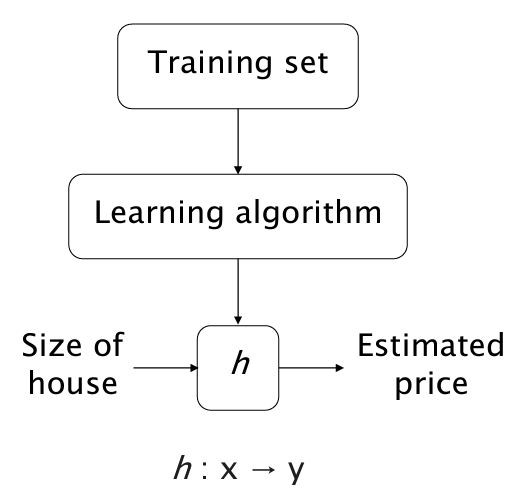
\includegraphics[scale=0.5]{img/model.png}
    \caption{Scheme for model construction (price prediction)}
\end{figure}

The figure above shows schematically the steps in order to produce a certain model for the analysed case-study. Very briefly, a \textbf{training set} is used by a \textbf{learning algorithm} to obtain an \textit{hypotesis} $h_\theta(x)$ which is later used for the prediction.\\
In the case we want to solve a \textbf{univariate linear regression problem} the hypotesis $h$ has got the shape:
\begin{equation}
    h_{\theta}(x)=\theta_0+\theta_1{x}
\end{equation}
where $\theta_0$ and $\theta_1$ are the parameters of the line.\footnote{
    We can imagine them as two handles to: move up/down the line ($\theta_0$) and to rotate it ($\theta_1$).
} We call \textit{univariate} the the problem since we have only one feature and it is a \textit{linear regression} because we want to predict the price (output) according to a line.\footnote{
    Note that in case of a \textbf{neural network} the parameters and the hypotesis assume a different notation. In particular the hypotesis becomes the \textit{predicted value} indicated with $\hat{y}$, the parameters are split in a \textbf{bias}, indicated with $b$ whose role is the one played by $\theta_0$, while the $\theta_i$, $i=1,...,n$ are the weights $w_i$
 }
\textbf{Question: How can we choose $\theta_0, \theta_1$?} Intuitively one can choose the parameters associated with the line $h_\theta(x)$ which is as closest as possible to the given $y$. Very often these parameters are the ones which solve the following problem: 
\begin{equation}\label{eq:ls1}
    \min_{\theta_0, \theta_1} \overbrace{\frac{1}{m} \sum_{i=1}^{m}{
        \frac{1}{2} \bigl(
            \underbrace{h_\theta(x^{(i)})}_{\textsf{predicted value}}-
            \underbrace{y^{(i)}}_{\textsf{actual value}}
            \bigr)^2
    }}^{\textsf{SQUARE ERROR COST FUNCTION}}
\end{equation}
The function $\frac{1}{2} (
    h_\theta(x^{(i)})-y^{(i)})^2$ is the \textsf{Loss}($h_\theta(x), y$) or \textsf{Cost}($h_\theta(x),y$).  If we call $J(\theta_0, \theta_1)$ the argument of the minimization problem the (\ref{eq:ls1}), the problem to solve can be expressed as
\begin{equation}\label{ls2}
    \min_{\theta_0, \theta_1} {J({\theta_0, \theta_1})}
\end{equation}
Summarizing: we want to perform a prediction using the hypotesis $h$ which is dependent on parameters $\theta_0, \theta_1$ which are issued by minimizing a certain functional $J(\theta_0, \theta_1)$. Let us investigate better on the role of $J$ in this supervised learning task.\\
At first -- for sake of simplicity -- we can eliminate a degree of freedom fixing the parameter $\theta_0$ to be (without loss of generality) $\theta_0=0$. For each choice of $\theta_1$ we will obtain a $h_{\theta_1}(x)$. If we compute $J(\theta_1)$ (for each $\theta$) will obtain a certain univariate function $J(\theta_1)$, the minimization of which will give us the \textit{optimal} $\theta_1$ parameter for our hypotesis. An example is shown in the following figure:

\begin{figure}[h]
    \centering
    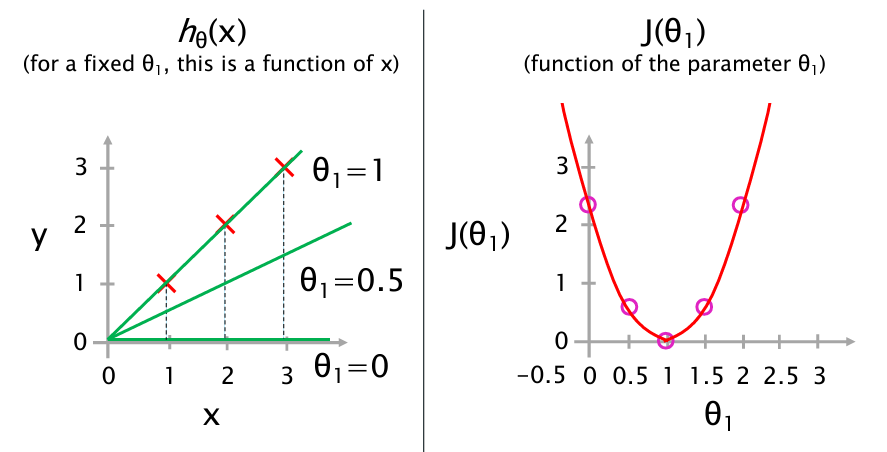
\includegraphics[scale=0.7]{img/J_univariate.png}
\end{figure}
\noindent
Analyzing the complete model, we have two degrees of freedom (DOF) since  $\theta_0, \theta_1$ can vary. In this case the functional to be minimized has to be represented in a 3D space, then we obtain a surface similar to one presented in the following figure:

\begin{figure}[h]\label{fig:surface}
   \centering
   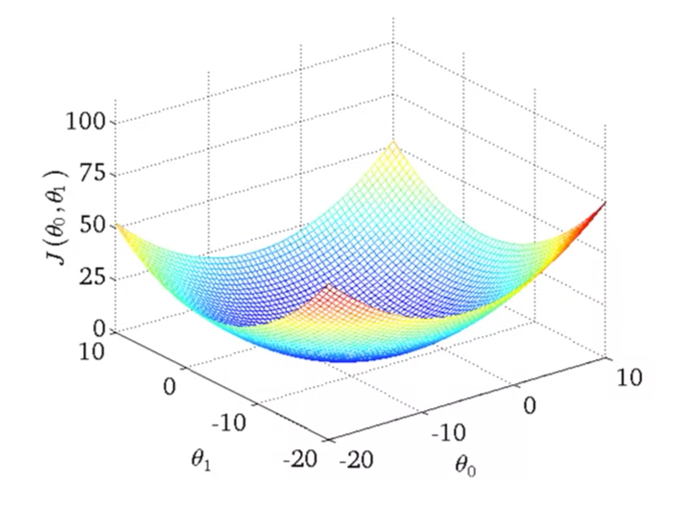
\includegraphics[scale=0.7]{img/J_bivariate.png} 
   \caption{Example of $J(\theta_0, \theta_1)$}
\end{figure}

In the common case of bivariate minimization problem one can use \textit{contour plot} which analyze the shape of the function at different heights. It is remarkable that points in the space $(\theta_0, \theta_1)$ which are on the same \textit{countour line} result in very different hypotesis. It is trivial to understand that,  in this case the minimum $J(\theta_0, \theta_1)$ is attained on the bottom of such a \textit{bowl-shaped} surface.

\begin{figure}[h]
    \centering
    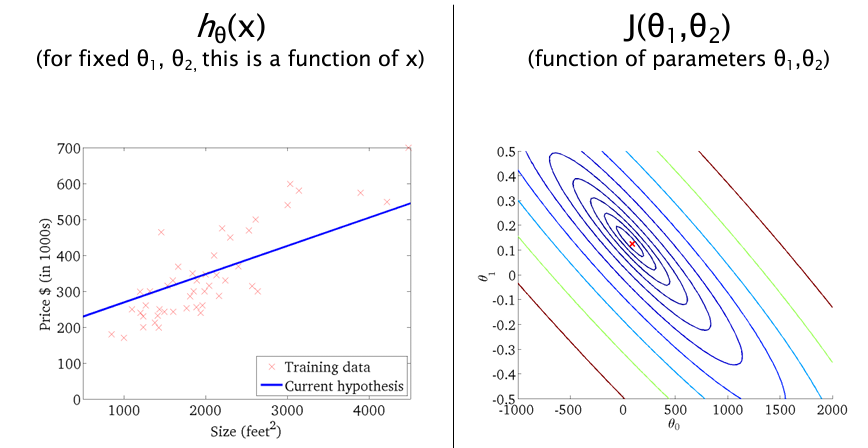
\includegraphics[scale=0.7]{img/contour.png}
\end{figure}

\section{Parameter learning: Gradient descent}
The objective here is to find a way to minimize a certain multivariate functional $J(\theta_1,..., \theta_n)$, the idea is using some methods that iteratively bring us to the minimum according to a certain criteria. In this paragraph we analyse the \textbf{Gradient Descent} algorithm, the main idea here is to start with some $\theta_0, \theta_1$\footnote{
    They are chosen either randomly or $\theta_i=0, \ \forall i$.
}, and keep changing them until $J$ evaluated at those parameters could reach (hopefully) the minimum, in the gradient descent this change is made up on the basis of the direction dictated by the \textbf{gradient of the functional} computed at the current parameters value (from which the name). The algorithm for GD is simply as follows:

\begin{figure}[h]
    \centering
    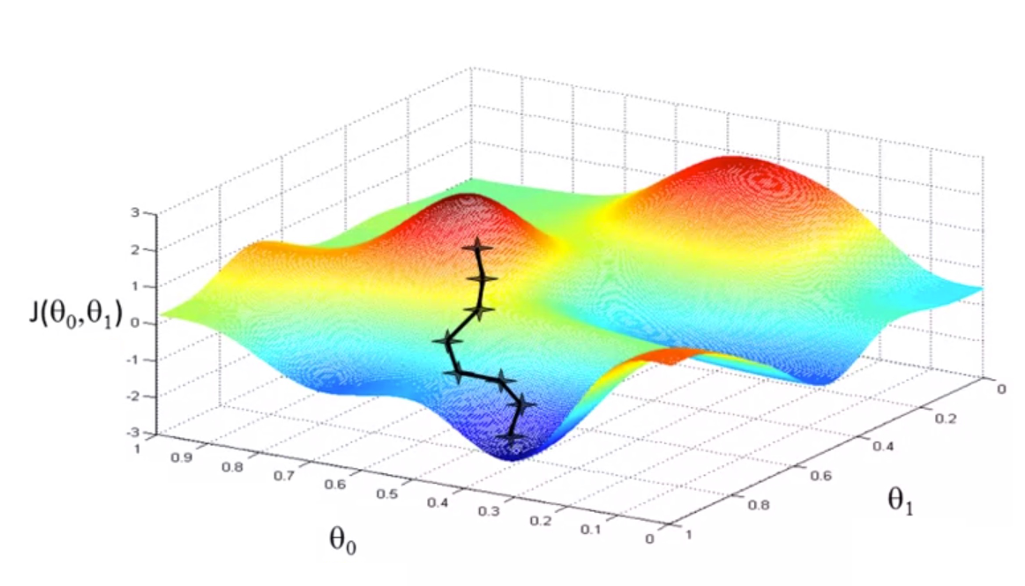
\includegraphics[scale=0.5]{img/nocvx_surf.png} 
\end{figure}

\begin{algorithm}[h]
    \caption{Gradient Descent}
    \begin{algorithmic}
        \While{!convergence}\\
           $\theta_j:=\theta_j-\alpha{\frac{\partial}{\partial{\theta_j}} J(\theta_0, \theta_1)}$
           \Comment{for $j$=0, $j$=1,...}
        \EndWhile
    \end{algorithmic}
\end{algorithm}

\noindent
The $:=$ symbol is associated with a \textit{simultaneous update}, note that if you put together for each $j$ the partial derivatives of $J$ you will obtain the gradient. The parameter $\alpha$ is called the \textbf{learning rate} and it must be properly chosen because:
\begin{itemize}
    \itemsep-0.2em
    \item If $\alpha$ is \textbf{too small}, then the convergence to the minimum (within a certain tolerance) could be very slow;
    \item If $\alpha$ is \textbf{too large} the algorithm can overshoot the minimum either failing to converge, or diverging.
\end{itemize}
Even when the learning rate is fixed the GD can converge to a (local) minimum since we are moving toward \textit{steep} directions which decrease the functional over time. If we apply the algorithm to the functional of the problem in (\ref{eq:ls1}) we obtain:
\begin{equation}
    \begin{aligned}
        &\theta_0=\theta_0-\alpha{\sum_{i=1}^{m}{(h_\theta(x^{(i)}-y^{(i)}))}}\\
        &\theta_1=\theta_1-\alpha{\sum_{i=1}^{m}{(h_\theta(x^{(i)}-y^{(i)}))} x^{(i)}}
    \end{aligned}
\end{equation}
this is known as \textbf{batch gradient descent} since for each step we use all the training samples. There are cases in which the minimization is particularly 'simple'. This happens when the functional is convex in $\theta$. Besides, for the class of convex functions a local minima is also a \textbf{global and only min}.

\section{Multivariate linear regression}
It is quite immediate to understand that the linear regression can be used also for a \textit{multivariate context} in which the samples are characterized by many features. In this context the hypotesis becomes:
\begin{equation}\label{eq:multivariate}
    h_\theta(x) = \theta_0{x_0}+\theta_1{x_1}+...+\theta_n{x_n}=\theta^T{x}
\end{equation}
In this case we have $n$ parameters and associated features $x_i$, so that the functional $J$ is function of $n$ parameters, in this case the partial derivatives to compute, obviously, will increase. Note that a \textit{fictitious} feature $x_0=1$ has been added with the purpose to employ a vector notation.\footnote{
    The great majority of tools and softwares which are used for machine learning exploit vector and matrices calculus to carry out their work.
}\\

\section{Data mean normalization}
Sometimes, before starting with the model construction, some preliminary operations are needed. For example, often it is better for the features being on a \textbf{similar scale}. In this  case we replace in each sample for each feature $x_i=x_i/s_i$ where $s_i$ can be either the range (max-min) for that feature or some index similar to variance/standard deviation.\\
Other times, one is supposed to normalize the data so that they can have a \textit{zero mean}. The trick here is replacing $x_i=x_i-\mu_i$, where $\mu_i$ is the mean for the $i$-th feature. Not rarely, you can find the two transformation combined such thet
\begin{equation}
    x_i=\frac{x_i-\mu_i}{s_i}
\end{equation}

\section{Debug of Gradient Descent algorithm}
The \textit{gradient algorithm} is clearly a descent method in the sense that -- being $k$ the $k$-th iteration -- it holds that $J(\theta_{k+1}) < J(\theta_{k})$, this is the same to state that the $J(\theta)$ function is required to be strictly decreasing. An \textbf{automatic convergence test} can be performed: for example the objective function $J$, had had a decreasing less than a certain threshold $\varepsilon=10^{-3}$ (for example).\\
Whether the algorithm is not working well the value for the \textbf{hyperparameter} $\alpha$ must be changed (for example decreasing it). One way to choose \textit{manually} $\alpha$ is by \textit{trial-error}\footnote{
    A more accurate method is the \textbf{backtracking line-search} which repeat some calculations until the so-called \textit{Armijo condition} is not met; however it requires that additive hypotesis are made on the regularity of the objective and its gradient.
}, choosing the $\alpha$ in a range and then plotting $J(\theta)$ as a function of the number of iterations. 

\begin{figure}[h]
    \centering
    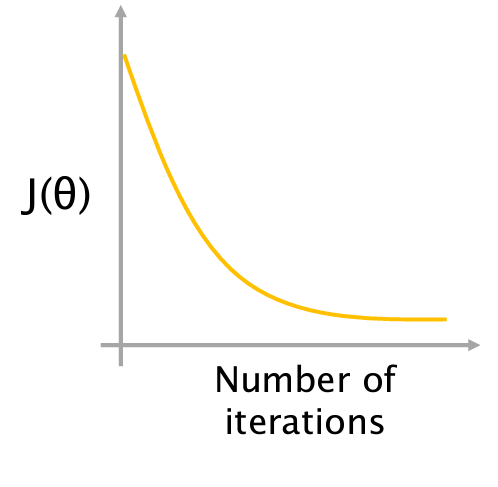
\includegraphics[scale=0.6]{img/alpha.png}
    \caption{Desired behaviour for $J(\theta)$ vs \# iterations}
\end{figure}
 
\section{Alternative to Gradient Descent}
There are alternative methods to gradient descent, for example the normal equation method which is derived by the analytical solution of the well-known \textbf{least-squares} problem. In this case $\theta$ is found by solving the system (normal equations):
\begin{equation}
    (X^T X)\theta = X^T{y}
\end{equation}
where the $X$ matrix contains the dataset features and $y$ is the vector with the "right answers". The solution of such a problem gives \textit{one-shot} the solution without proceeding by step as in the case  of gradient descent. The main limitation of such a method is the inversion of the matrix $X^T X$, which could be significantly slow if $n$ (number of features and parameters) is very large.\footnote{
    It is sufficient to think about the number of parameters involved in a problem of image classification. They are in a number of 3 billion for an RGB $1000\times1000$ image. 
}

\section{Polynomial regression}
Not rarely can happen that a linear hypotesis is not satisfactory for our task of regression and so could be useful to introduce some other features by doing the so-called \textit{handcrafting}. The derived features can be nonlinear, and specifically polynomial, combination of the available features. In the case of the price predition the handcrafted features could be for example the square of the size and the cube of the size. 


